\documentclass{article}

\usepackage{fancyhdr}
\usepackage{extramarks}
\usepackage{amsmath}
\usepackage{amsthm}
\usepackage{amssymb}
\usepackage{amsfonts}
\usepackage{tikz}
\usepackage{physics}
\usepackage[plain]{algorithm}
\usepackage{algpseudocode}
\usepackage{graphicx,wrapfig,lipsum}
\usetikzlibrary{automata,positioning}

%
% Basic Document Settings
%

\topmargin=-0.45in
\evensidemargin=0in
\oddsidemargin=0in
\textwidth=6.5in
\textheight=9.0in
\headsep=0.25in

\linespread{1.1}

\pagestyle{fancy}
\lhead{\hmwkAuthorName}
\chead{\hmwkClass\ : \hmwkTitle}
\rhead{\firstxmark}
\lfoot{\lastxmark}
\cfoot{\thepage}

\renewcommand\headrulewidth{0.4pt}
\renewcommand\footrulewidth{0.4pt}

\setlength\parindent{0pt}

%
% Create Problem Sections
%
\newcommand{\be}{\begin{equation}}
\newcommand{\ee}{\end{equation}}
\newcommand{\bes}{\begin{equation*}}
\newcommand{\ees}{\end{equation*}}
\newcommand{\bea}{\begin{flalign*}}
\newcommand{\eea}{\end{flalign*}}


\newcommand{\enterProblemHeader}[1]{
    \nobreak\extramarks{}{Problem \arabic{#1} continued on next page\ldots}\nobreak{}
    \nobreak\extramarks{Problem \arabic{#1} (continued)}{Problem \arabic{#1} continued on next page\ldots}\nobreak{}
}

\newcommand{\exitProblemHeader}[1]{
    \nobreak\extramarks{Problem \arabic{#1} (continued)}{Problem \arabic{#1} continued on next page\ldots}\nobreak{}
    \stepcounter{#1}
    \nobreak\extramarks{Problem \arabic{#1}}{}\nobreak{}
}

\setcounter{secnumdepth}{0}
\newcounter{partCounter}
\newcounter{homeworkProblemCounter}
\setcounter{homeworkProblemCounter}{1}
\nobreak\extramarks{Problem \arabic{homeworkProblemCounter}}{}\nobreak{}

%
% Homework Problem Environment
%
% This environment takes an optional argument. When given, it will adjust the
% problem counter. This is useful for when the problems given for your
% assignment aren't sequential. See the last 3 problems of this template for an
% example.
%
\newenvironment{homeworkProblem}[1][-1]{
    \ifnum#1>0
        \setcounter{homeworkProblemCounter}{#1}
    \fi
    \section{Problem \arabic{homeworkProblemCounter}}
    \setcounter{partCounter}{1}
    \enterProblemHeader{homeworkProblemCounter}
}{
    \exitProblemHeader{homeworkProblemCounter}
}

%
% Homework Details
%   - Title
%   - Due date
%   - Class
%   - Section/Time
%   - Instructor
%   - Author
%

\newcommand{\hmwkTitle}{Assignment\ \#2}
\newcommand{\hmwkDueDate}{Due on 11th September, 2018}
\newcommand{\hmwkClass}{Fluid Mechanics}
\newcommand{\hmwkClassTime}{}
\newcommand{\hmwkClassInstructor}{}
\newcommand{\hmwkAuthorName}{\textbf{Aditya Vijaykumar}}

%
% Title Page
%

\title{
    %\vspace{2in}
    \textmd{\textbf{\hmwkClass:\ \hmwkTitle}}\\
    \normalsize\vspace{0.1in}\small{\hmwkDueDate\ }\\
%    \vspace{3in}
}

\author{\hmwkAuthorName}
\date{}

\renewcommand{\part}[1]{\textbf{\large Part \Alph{partCounter}}\stepcounter{partCounter}\\}

%
% Various Helper Commands
%

% Useful for algorithms
\newcommand{\alg}[1]{\textsc{\bfseries \footnotesize #1}}

% For derivatives
\newcommand{\deriv}[1]{\frac{\mathrm{d}}{\mathrm{d}x} (#1)}

% For partial derivatives
\newcommand{\pderiv}[2]{\frac{\partial}{\partial #1} (#2)}

% Integral dx
\newcommand{\dx}{\mathrm{d}x}

% Alias for the Solution section header
\newcommand{\solution}{\textbf{\large Solution}}

% Probability commands: Expectation, Variance, Covariance, Bias
\newcommand{\E}{\mathrm{E}}
\newcommand{\Var}{\mathrm{Var}}
\newcommand{\Cov}{\mathrm{Cov}}
\newcommand{\Bias}{\mathrm{Bias}}

\begin{document}

\maketitle

%\pagebreak

\begin{homeworkProblem}
    \textbf{Part (a)}\\
   	Given the assumptions, we can effectively consider the two volcanoes as sources/sinks in 2 dimensions. At some height $ h $, this then makes $ mh $ and $ nh $ the strength of the sources respectively. Consider the volcano at $ (0,0) $ to have strength $ m/h $ and the one at $ (d,0) $ to have $ n/h $. At some point $ (x,y) $, the velocity purely due to each of the volcanoes is given by,
   	\begin{equation*}
   	\vb{v}_1 = \frac{m}{2\pi h(x^2 + y^2)}(x\vu{x} + y \vu{y}) \qq{and} \vb{v}_2 = \frac{n}{2\pi h((x-d)^2 + y^2)}((x-d)\vu{x} + y \vu{y})
   	\end{equation*}
   	The final velocity field is just the vector addition,
   	\begin{equation*}
   	\vb{v} = \vb{v}_1 + \vb{v}_2= \frac{1}{2\pi h}\qty[\qty(\frac{mx}{x^2+y^2} +\frac{n(x-d)}{(x-d)^2 + y^2})\vu{x} + \qty(\frac{my}{x^2+y^2} +\frac{ny}{(x-d)^2 + y^2})\vu{y} ]
   	\end{equation*}
   	
   	\textbf{Part (b)}\\
   	Obviously, $ h $ is not truly constant. There will be some additional force generated due to the pressure difference, which will then require us to solve the full Navier-Stokes equation to find the velocity field.
   	\\
   	
   	\textbf{Part (c)}\\
   	If $ n<0 $, the second volcano is basically sucking in ash, and hence will act as a sink. The field sketches for both parts is given below
   	
   	\begin{figure}[!h]
   		\caption{Figures - L: Part (a) and R: Part (c)}
   		\centering
   		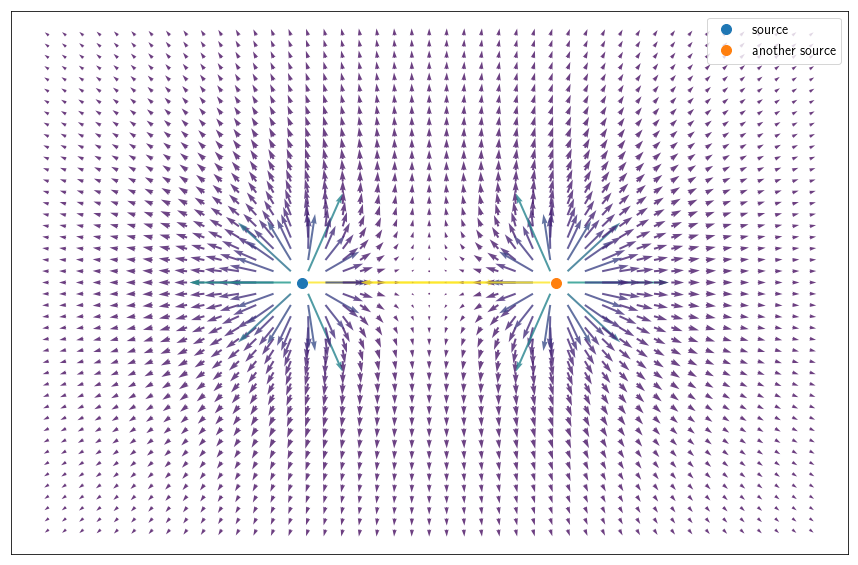
\includegraphics[scale=0.26]{source.png}
   		\hspace{0.1in}
   		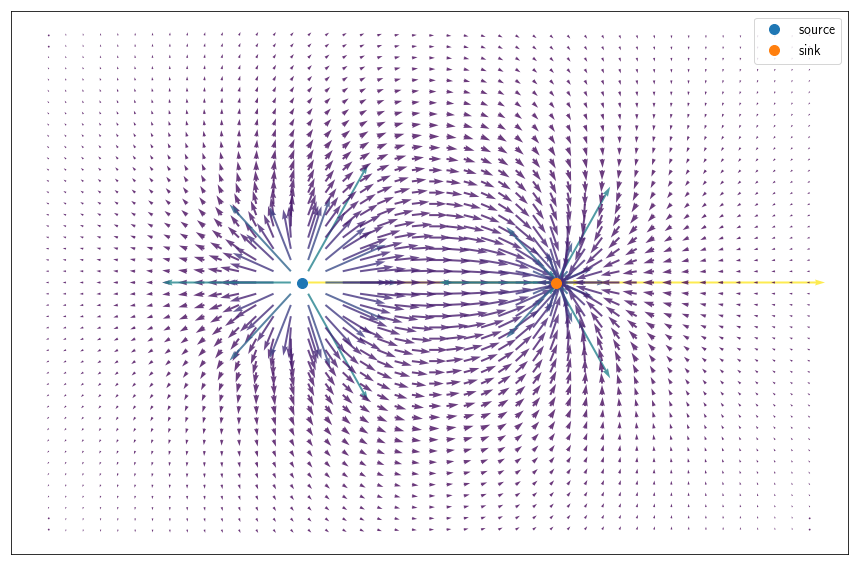
\includegraphics[scale=0.26]{sink.png}
   	\end{figure}
\end{homeworkProblem}

\begin{homeworkProblem}
	\textbf{Part (a)}\\
	\begin{wrapfigure}{l}{0.5\textwidth}
		\begin{center}
			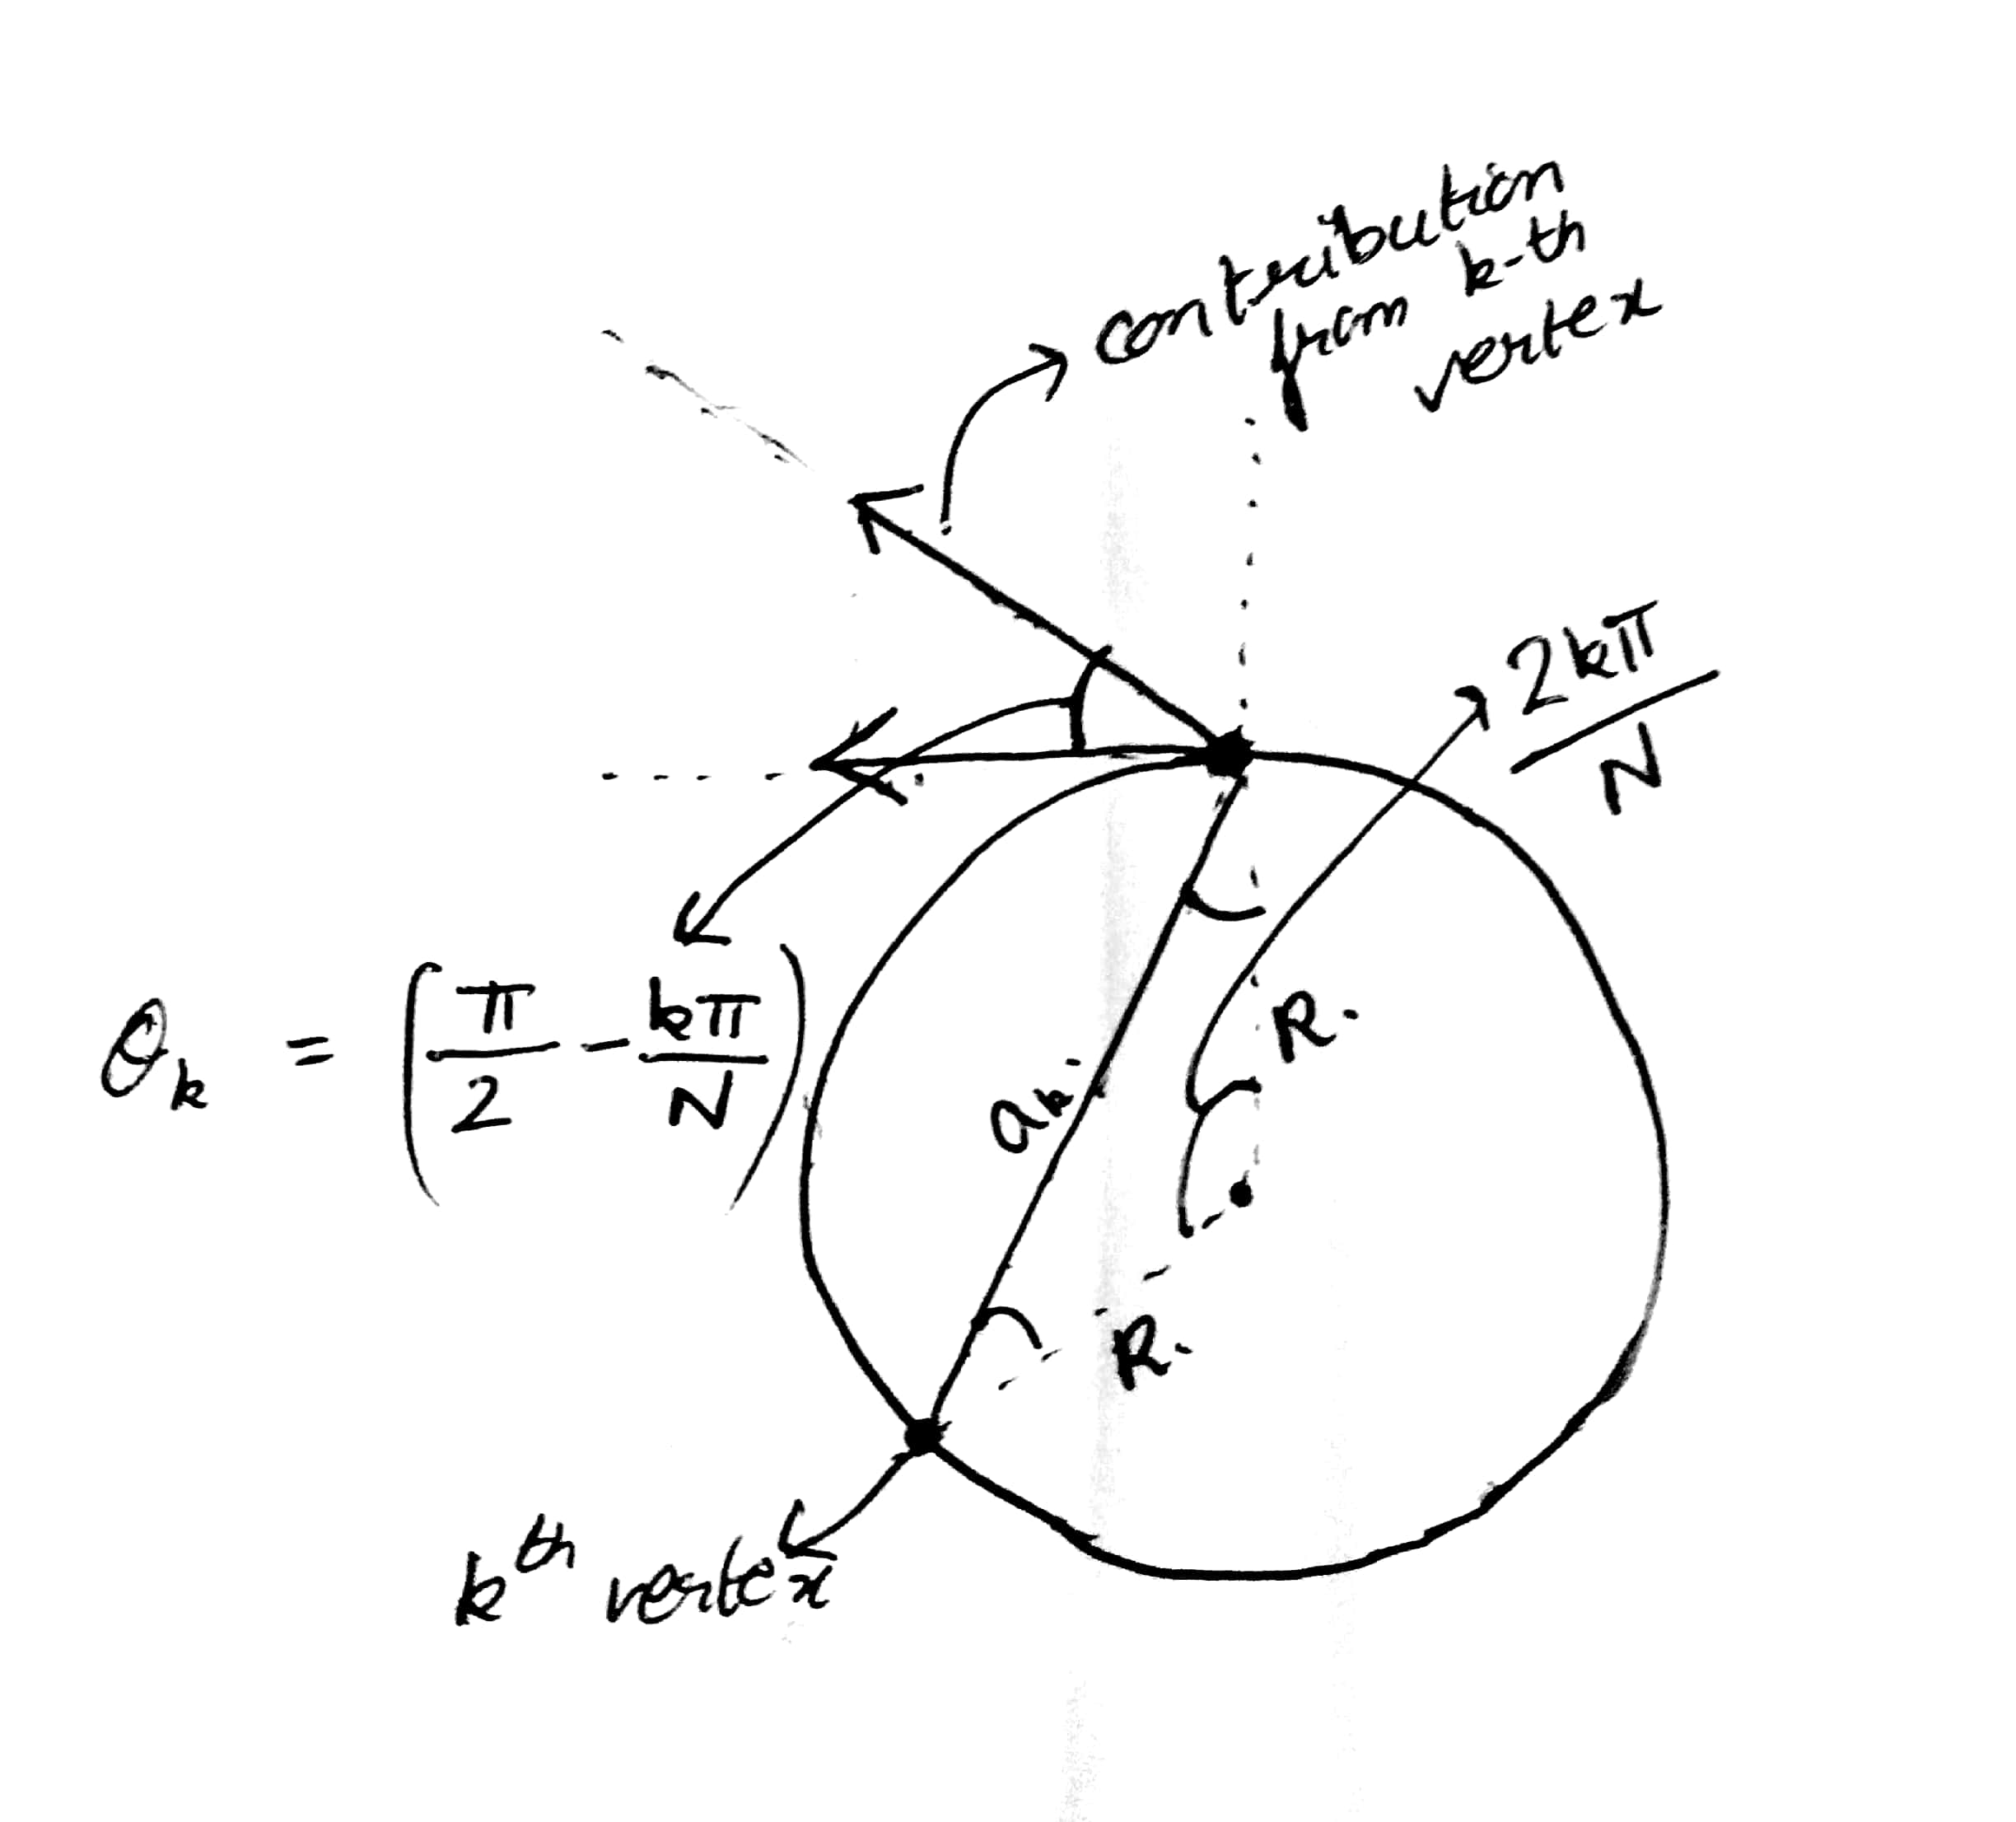
\includegraphics[scale=0.08]{1a.jpg}
		\end{center}
	\end{wrapfigure}
	For a regular polygon with $ N $ sides, each side will subtend an angle $ \dfrac{2\pi}{N} $ at the centre. As the problem is symmetric, it is enough to solve for the motion of one point vortex.
	
	Considering a single vertex of the polygon, we can see that the motion will have contributions from the other $ N-1 $ vertices. As shown in the figure, only the horizontal components of these contributions will survive. Hence resultant tangential velocity will be given by,
	\begin{equation*}
	v = \sum_{k = 1}^{N-1} \dfrac{\Gamma}{2\pi a_k }\cos \theta_k
	\end{equation*}
	where $ k $ is the serial number of vertices starting anticlockwise from the vertex under consideration. It is evident from the figure that, 
	\begin{equation*}
	\theta_k = \dfrac{\pi}{2} - \dfrac{k\pi}{N} \qq{and} a_k = 2 R \sin \dfrac{k\pi}{N}
	\end{equation*}
	where $ R $ is the distance of each vertex from the centre. Substituting this in the expression for velocity, and noting that $ \l = 2R \sin \dfrac{\pi}{N} $ where $ l $ is side length
	\begin{equation*}
	v = \dfrac{(N-1)\Gamma}{4\pi R} = \dfrac{(N-1)\Gamma  \sin \dfrac{\pi}{N} }{2\pi l}
	\end{equation*}
	The time period $ T $ is given by,
	\begin{equation*}
	\boxed{T = \dfrac{2\pi R}{v} = \dfrac{8 \pi^2 R^2}{(N-1)\Gamma} = \dfrac{2 \pi^2 l^2}{(N-1)\Gamma \sin^2 \dfrac{\pi}{N}}}
	\end{equation*}
	
	\textbf{Part (b)}\\
	As the expression for time period we have got is pretty simple, there is no need to solve this problem on the computer.
	
	\begin{equation*}
	\boxed{\qq{For $ N=4 $;} T = \dfrac{8 \pi^2 R^2}{3 \Gamma}}
	\end{equation*}
	\begin{equation*}
	\boxed{\qq{For $ N=10 $;} T = \dfrac{8 \pi^2 R^2}{9 \Gamma}}
	\end{equation*}
	
	\textbf{Part (c)}\\
	For a non-identical polygon, the flow will not be circular, and could follow some chaotic trajectory.
\end{homeworkProblem}

\end{document}
